To save computational effort, the axisymmetry is exploited in the simulation of the capillary, and only a wedge is simulated. The angle of the wedge is \(5^\circ\). Furthermore, water is assumed as the liquid medium and air as the gaseous medium, both at \(25^\circ\) Celsius. The corresponding material properties are listed in the following table.

\begin{table}[h]
\centering
\caption{Physical properties}
\label{tab:physicalProperties_CaseSetup}
\begin{tabular}{lll}
fluid & density ($\frac{kg}{m^3}$) & kinematic viscosity $\frac{m^2}{s}$ \\ \hline
water & $1000$                     & $1.00E-06$                          \\
air   & $1$                        & $1.00E-05$                          \\ 
\end{tabular}
\end{table}
\todo[inline]{insert table}

The surface tension between water and air is \(0.072 N/m\), and the interface thickness \( \epsilon \) was chosen to be approximately \(1.7 nm\), corresponding to the physical interface thickness. Mobility is a factor in the phase-field simulation that is difficult to determine. Jacqmin \cite{jacqmin1999CalculationTwoPhaseNavier} suggested an asymptotic behavior for \( \kappa \) of 
\begin{equation}
    \kappa = \mathcal{O}(\epsilon^{\delta})
\end{equation}
and showed that \( 1 \leq \delta < 2 \). For this work, a value of \( \kappa = 4 \times 10^{-18} \) was used.

Simulations were conducted for various contact angles to investigate the influence of capillary rise depending on the contact angle. The initial conditions for each of these simulations were the same. The computational grid was chosen such that the elements in the axial direction. \todo[inline]{elaborate}

\begin{figure}[h]
    \centering
    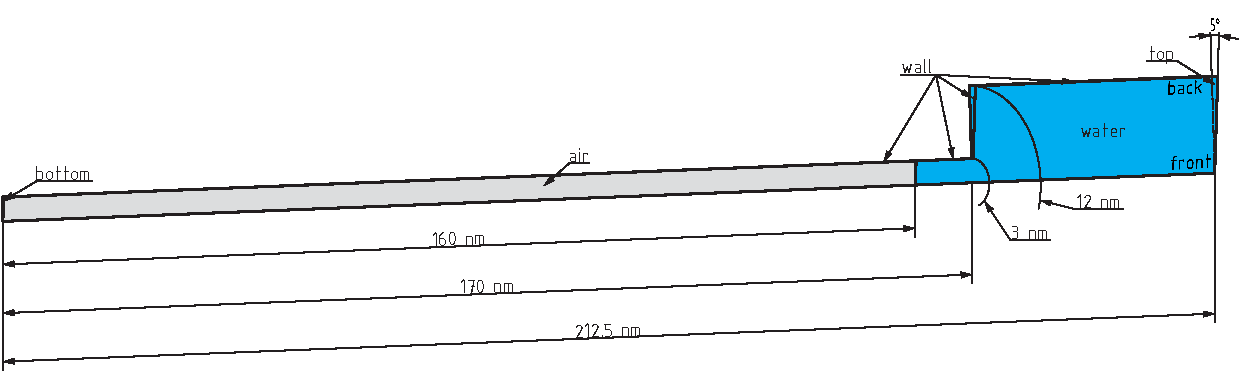
\includegraphics[width=.9\textwidth]{Pictures/Cap_5DEG.pdf}
    \caption{Wedge-shaped case setup}
    \label{fig: wedge_caseSetup}
\end{figure}

In Figure \ref{fig: wedge_caseSetup}, both the dimensions of the wedge and the names of the surfaces that have been assigned with boundary conditions are shown. Furthermore, it can be seen which part of the capillary is already filled with water (blue area) and which part is filled with air (gray area). The surfaces labeled \texttt{front} and \texttt{back} represent the opposing faces of the wedge. The surfaces \texttt{top} and \texttt{bottom} have a zero-gradient boundary condition and a pressure of \(0\,Pascal\). At the wall, the no-slip condition applies, and for the order parameters, an equilibrium boundary condition is used. In this work, the usability and effects of the out-of-equilibrium boundary condition are examined as well. Additional simulations were conducted with the same setup as before, but with the activated boundary condition. \todo{ref to chapter ooEBC}
\section{Discretization}
Da es sich um eine relativ simple geometrie handelt, wurde die Geometrie direkt in der \texttt{blockMeshDict}- Datei erstellt. Die Netzdichte wurde so gewählt, dass die Kantenlänge der Kontrollvolumen $0.1nm$ entsprechen. Dadurch können mögliche Probleme durch geringe Kontaktwinkel minimiert werden. Simulationen mit großem Winkel wurden ebenfalls mit gleichem Rechnetz simuliert, um eine gute vergleichbarbeit gewährleisten zu können. \todo{we used an other geometry. How do i write it then?new image with new text? }




One of the significant advantages of simulation is the ability to examine areas that are difficult or impossible to measure in reality. For each of the simulations, several values were extracted to assist in the later evaluation and assessment of the simulation. These include the acting viscous or capillary forces.



